\documentclass[12pt,a4paper]{exam}
\usepackage[utf8]{inputenc}
\usepackage[T1]{fontenc}
\usepackage{amsmath}
\usepackage{amsfonts}
%\usepackage{amssymb}
\usepackage{graphicx}
\usepackage{geometry}
\usepackage{enumitem}

\geometry{a4paper, margin=2cm}

\usepackage{cprotect}

\usepackage{xcolor}
\definecolor{maroon}{cmyk}{0, 0.87, 0.68, 0.32}
\definecolor{halfgray}{gray}{0.55}
\definecolor{ipython-frame}{RGB}{207, 207, 207}
\definecolor{ipython-bg}{RGB}{247, 247, 247}
\definecolor{ipython-red}{RGB}{186, 33, 33}
\definecolor{ipython-green}{RGB}{0, 128, 0}
\definecolor{ipython-cyan}{RGB}{64, 128, 128}
\definecolor{ipython-purple}{RGB}{170, 34, 255}

\usepackage{listings}
\lstdefinelanguage{iPython}{
	morekeywords={access,and,del,except,exec,in,is,lambda,not,or,raise},
	morekeywords=[2]{for,print,abs,all,any,basestring,bin,bool,bytearray,callable,chr,classmethod,cmp,compile,complex,delattr,dict,dir,divmod,enumerate,eval,execfile,file,filter,float,format,frozenset,getattr,globals,hasattr,hash,help,hex,id,input,int,isinstance,issubclass,iter,len,list,locals,long,map,max,memoryview,min,next,object,oct,open,ord,pow,property,range,reduce,reload,repr,reversed,round,set,setattr,slice,sorted,staticmethod,str,sum,super,tuple,type,unichr,unicode,vars,xrange,zip,apply,buffer,coerce,intern,elif,else,if,continue,break,while,class,def,return,try,except,import,finally,try,except,from,global,pass, True, False},
	sensitive=true,
	morecomment=[l]\#,%
	morestring=[b]',%
	morestring=[b]",%
	moredelim=**[is][\color{black}]{@@}{@@},
	identifierstyle=\color{black}\footnotesize\ttfamily,
	commentstyle=\color{ipython-cyan}\footnotesize\itshape\ttfamily,
	stringstyle=\color{ipython-red}\footnotesize\ttfamily,
	keepspaces=true,
	showspaces=false,
	showstringspaces=false,
	rulecolor=\color{ipython-frame},
	frame=single,
	frameround={t}{t}{t}{t},
	backgroundcolor=\color{ipython-bg},
	basicstyle=\footnotesize\ttfamily,
	keywordstyle=[2]\color{ipython-green}\bfseries\footnotesize\ttfamily, 
	keywordstyle=\color{ipython-purple}\bfseries\footnotesize\ttfamily
}

\lstdefinelanguage{iOutput} {
	sensitive=true,
	identifierstyle=\color{black}\small\ttfamily,
	stringstyle=\color{ipython-red}\small\ttfamily,
	keepspaces=true,
	showspaces=false,
	showstringspaces=false,
	rulecolor=\color{ipython-frame},
	basicstyle=\small\ttfamily,
}

\lstnewenvironment{ipython}[1][]{\lstset{language=iPython,mathescape=true,escapeinside={*@}{@*}}%
}{%
}

\lstnewenvironment{ioutput}[1][]{\lstset{language=iOutput,mathescape=true,escapeinside={*@}{@*}}%
}{%
}


\title{Financial Market Course 25/26\\ Exam}
\author{Prof. Simone Freschi, Prof. Matteo Sani}
\date{$4^{\mathrm{th}}$ September 2026}

\printanswers
%\noprintanswers
\begin{document}
\maketitle

\begin{center}
\fbox{\fbox{\parbox{5.5in}{
Answer the questions in the provided spaces. If you run out of room for an answer, continue on the page back.}}}
\end{center}

\begin{center}
\vspace{5mm}
\makebox[0.75\textwidth]{Student's name:\enspace\hrulefill}
\end{center}

\section*{Questions}
\vspace{.5cm}
\begin{questions}

\question 
Describe what are the main characteristics of a Repo Contract.
\begin{parts}
	\part In the chart I is described the delivery Basket of the BTP Future September 2026 (IKU6) which is currently trading at 114.20. The bond BTPS 3.65 August 2035 is the cheapest to deliver with a price of 97.03 and a conversion factor of 0.8452. Describe if there is an arbitrage opportunity and what kind of strategy would you implement. (\textit{hint}: check the basis and use the cash and carry strategy)
\end{parts}

\makeemptybox{5cm}
\begin{figure}[htb]
	\centering
	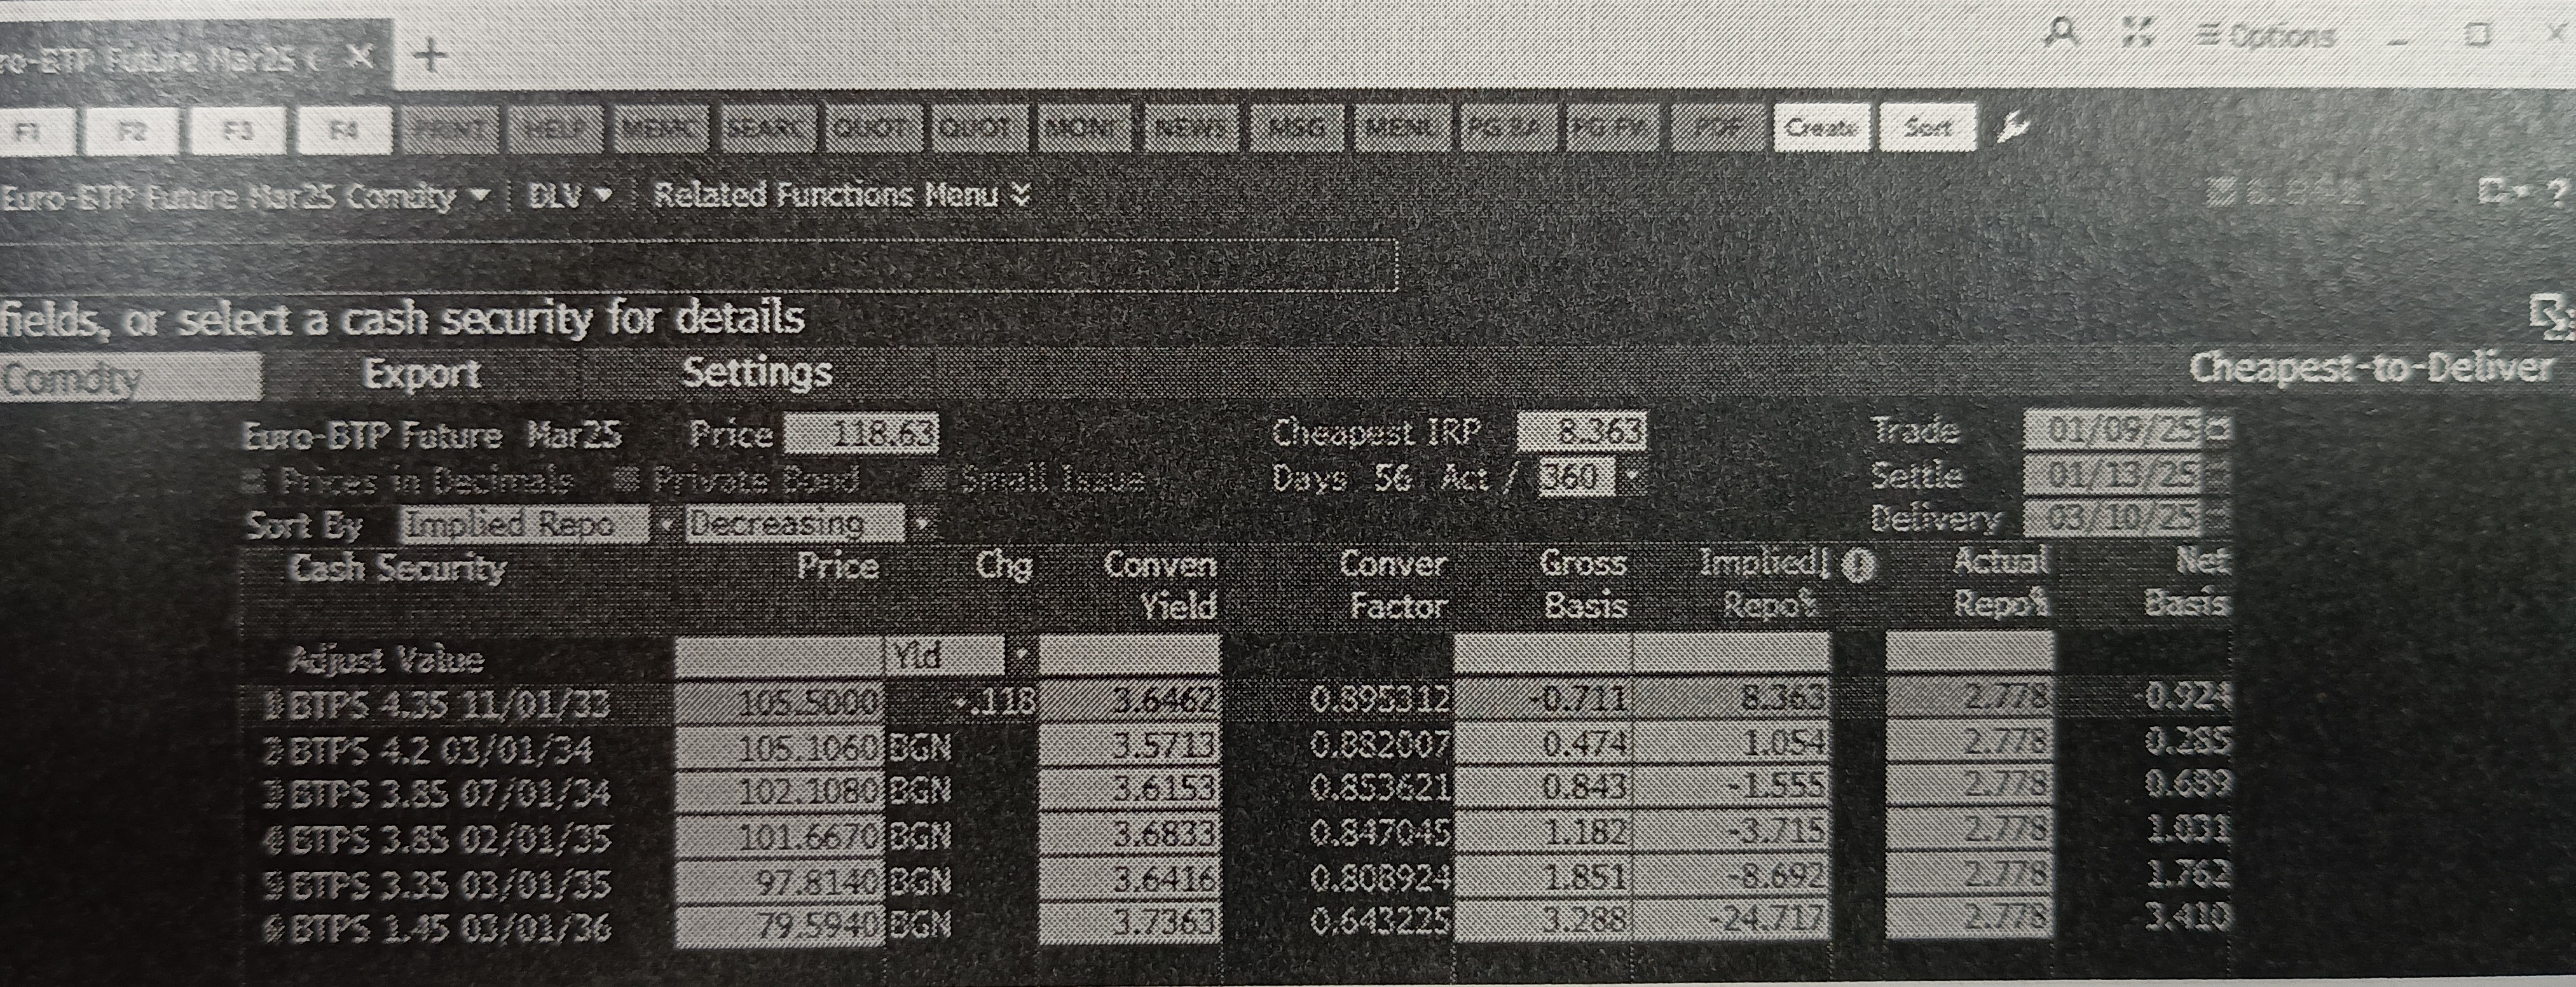
\includegraphics[width=0.9\linewidth]{immagine_compito_27_01_2026}
	\caption{BTP September 2026 Futures}
\end{figure}

\begin{figure}[htb]
	\centering
	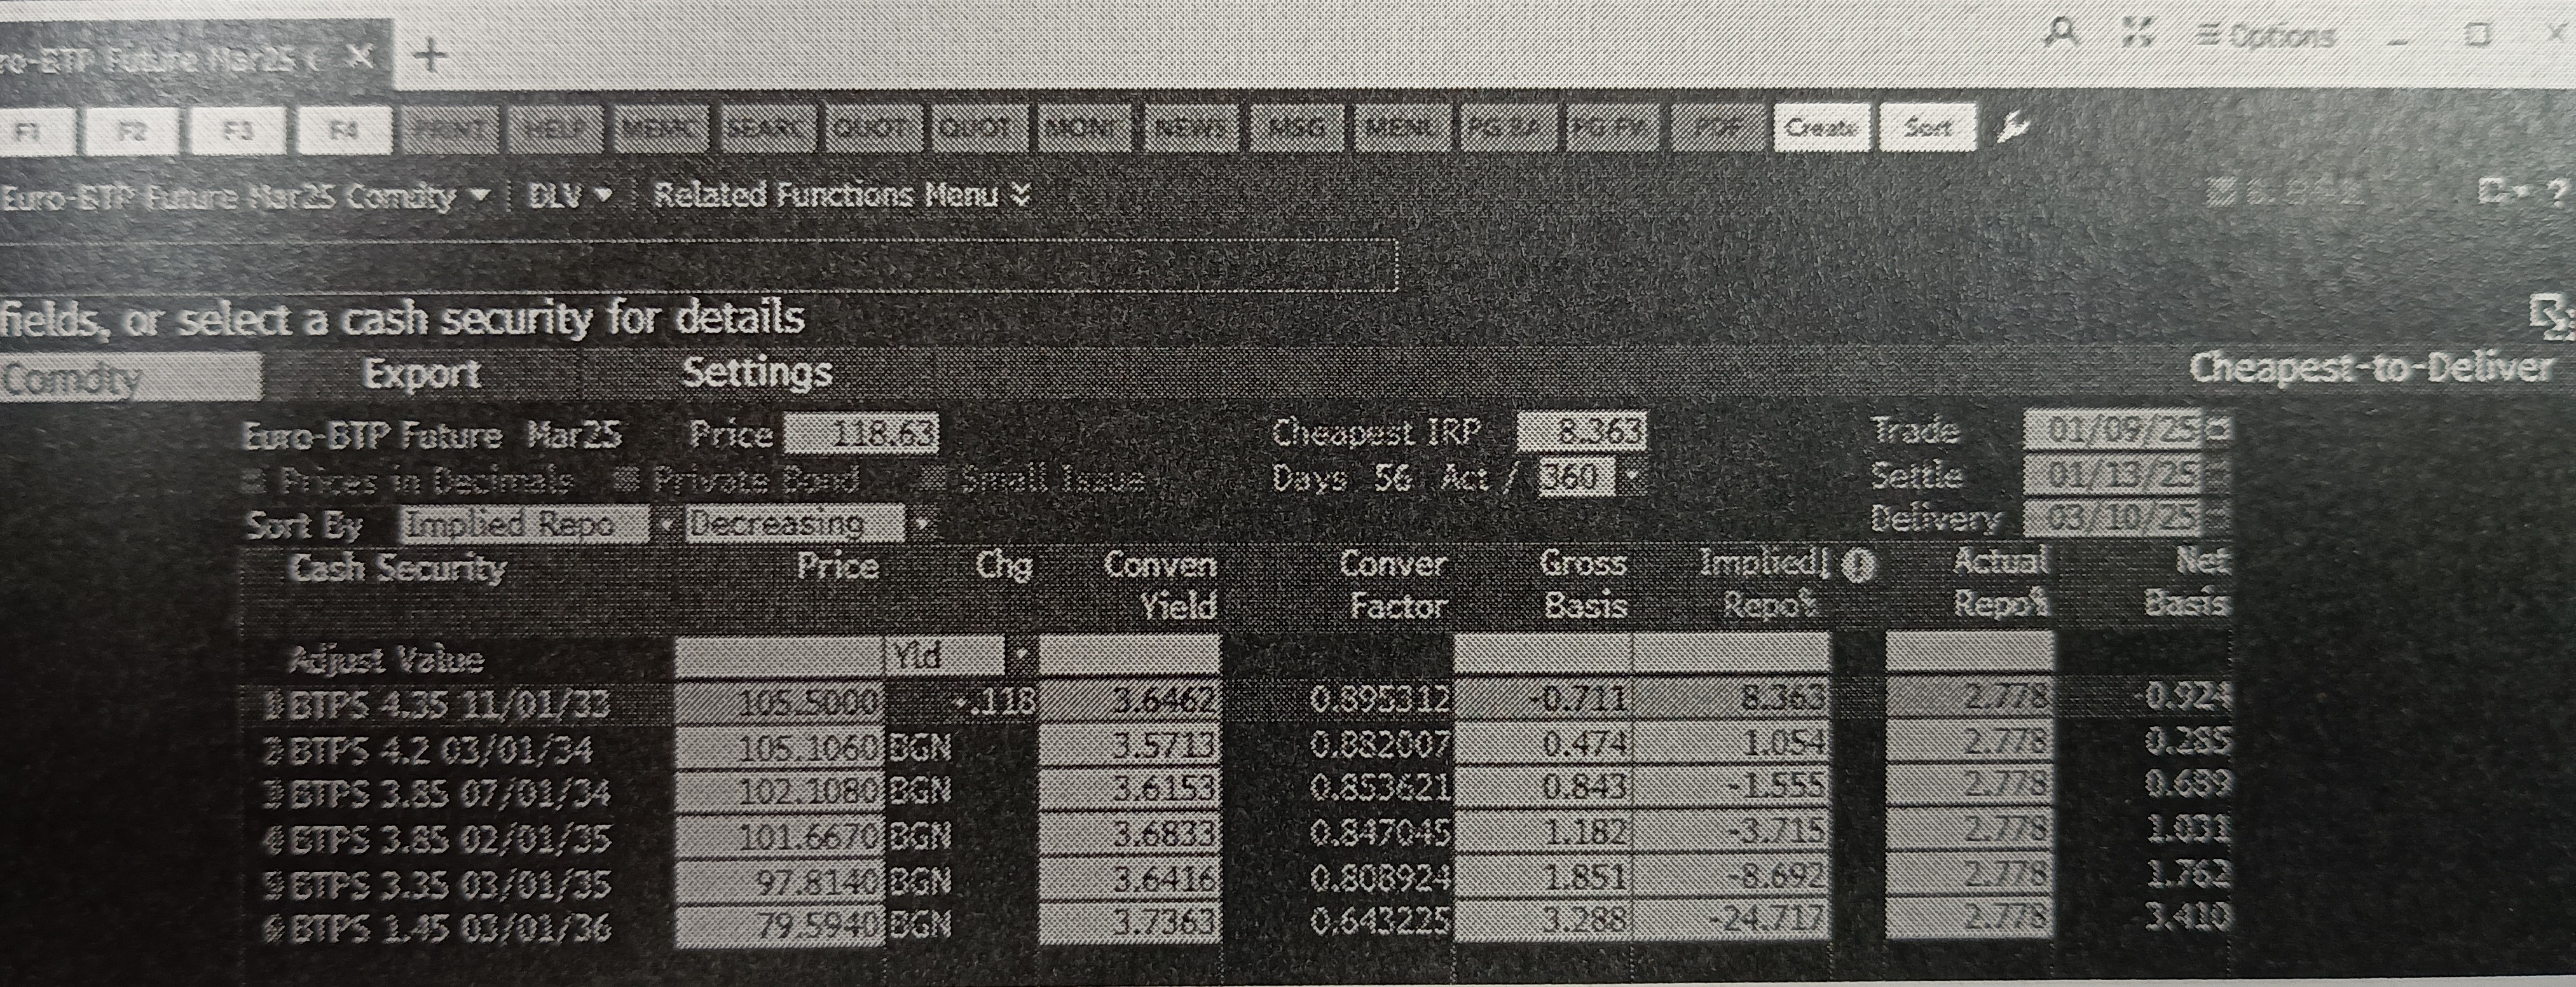
\includegraphics[width=0.9\linewidth]{immagine_compito_27_01_2026}
	\caption{ETF on TIPS}
\end{figure}

%\fillwithdottedlines{5cm}
\begin{solution}
\end{solution}

\question
Inflation Linked Bonds
\begin{parts}
	\part Describe the price in real terms and nominal terms of an Inflation Linked Bond.
	\part Look at the two Bloomberg charts 2 and 3: TIP US (the ETF on US Treasury Inflation Protected with duration of 6.7 years) and USGG10YR Index (US nominal 10Y yield lhs), overlaid with USSWIT10, (thje 10Y inflation swap rate rhs), both Year To Date 2026.
	TIP US has fallen from roughly 112 in late February to below 107 (minus 5\% by September, while the nominal 10Y yield (USGG10YR) has risen from about 4.2\% to nearly 4.8\% over the same period, and the 10Y inflation has moderately increasing (15 bps) since Ytd. According to the previous formula explain if and why the behaviour of the ETF is consisent with ehe market.
\end{parts}

\begin{figure}[htb]
	\centering
	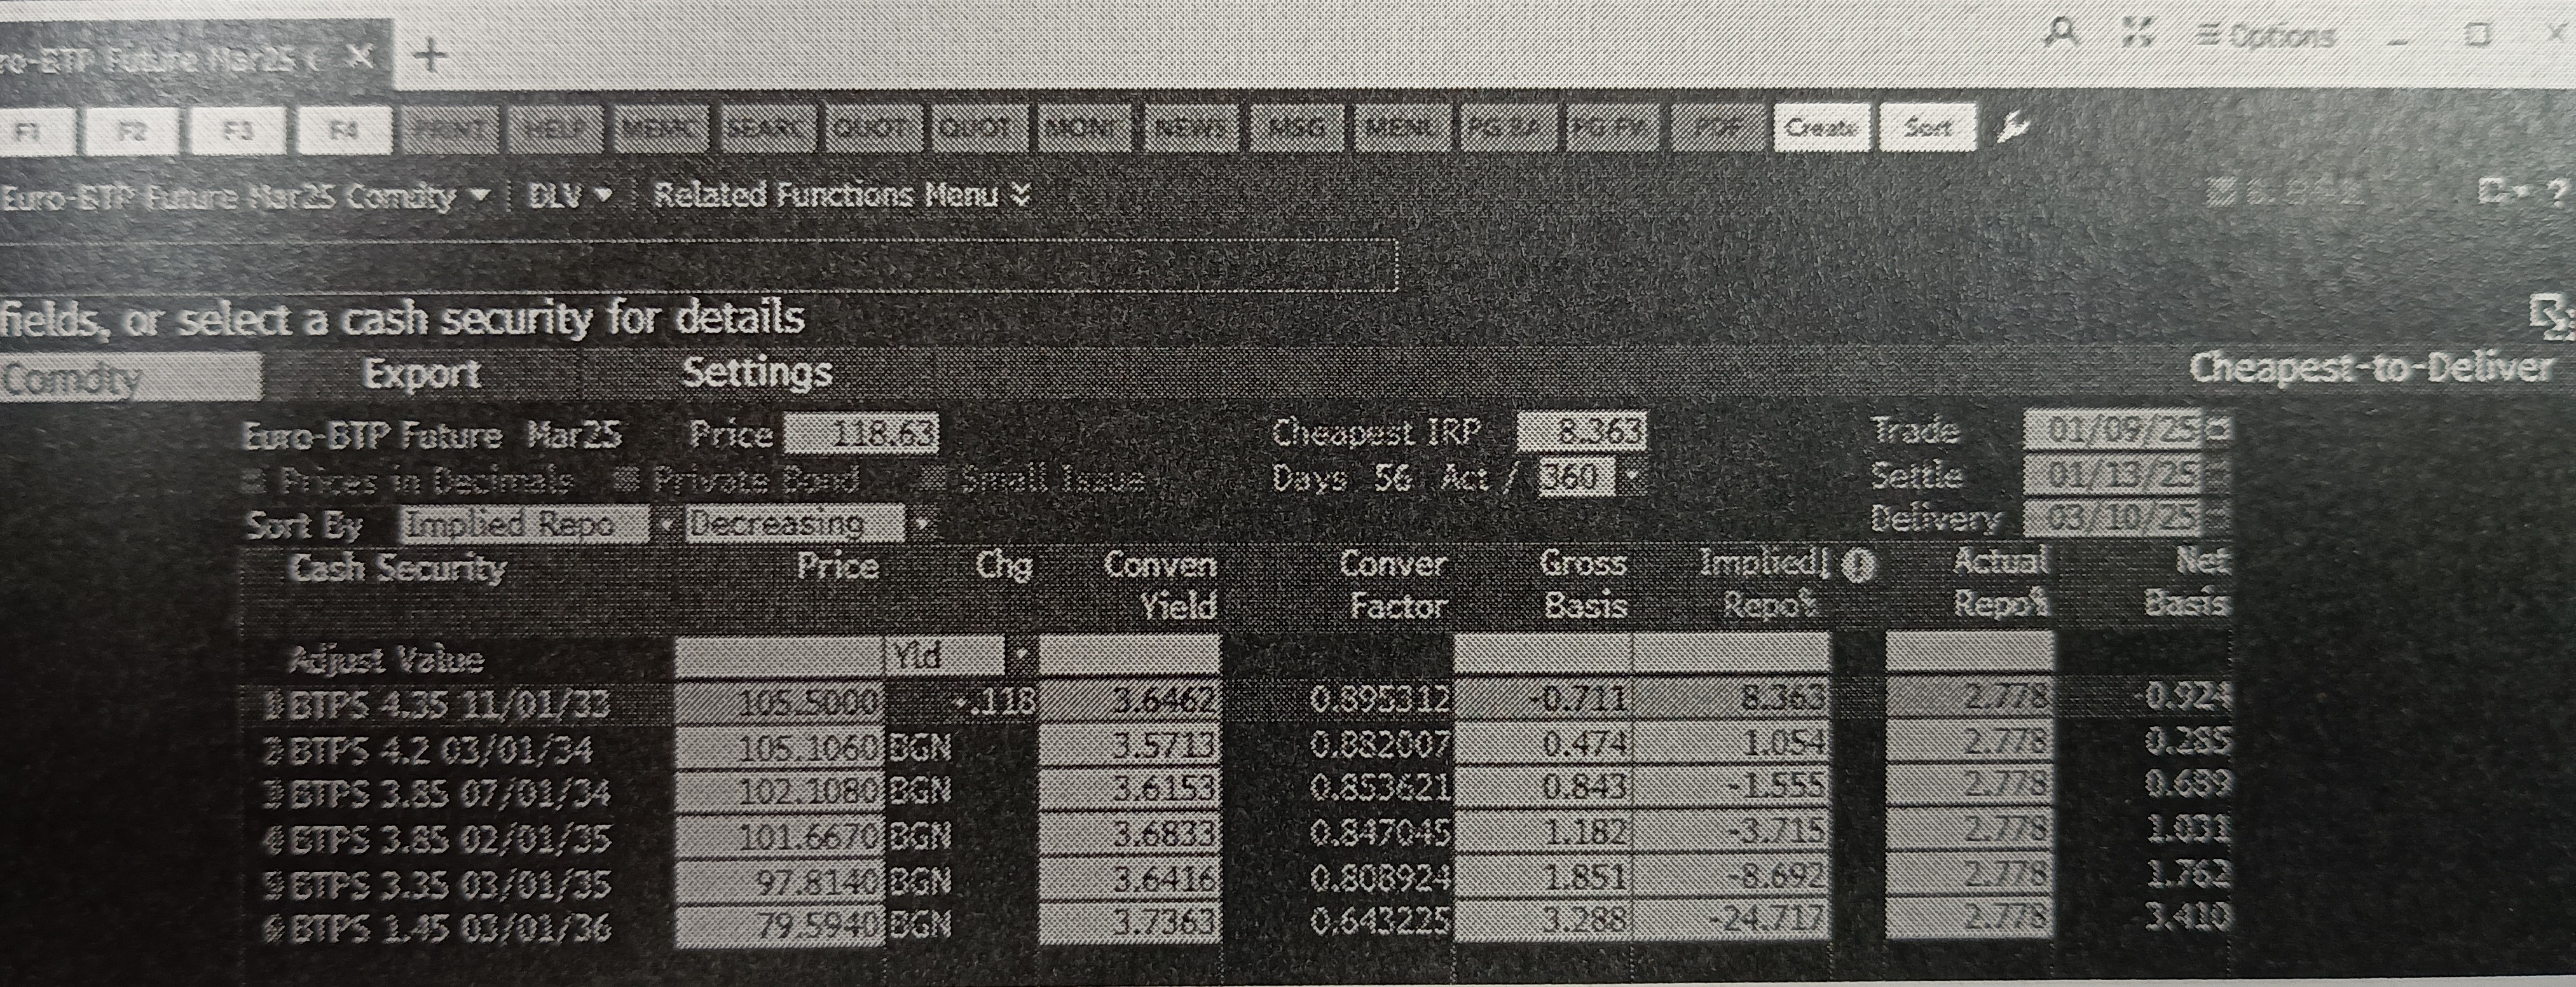
\includegraphics[width=0.9\linewidth]{immagine_compito_27_01_2026}
	\caption{10y nominal rate and 10y inflation swap.}
\end{figure}

\makeemptybox{5cm}
%\fillwithdottedlines{5cm}
\begin{solution}
\end{solution}

%%%%%%%%%%%%%%%%%%%%%%%%%%%%%%%%%%%%%
\question 
Describe the equation for the return attribution model by Brinson, Hood and Beebower (BHB).
\begin{parts}
	\part Explain the difference between Allocation Effect and Security Selection Effect.
	\part Imagine that your portfolio is underweight Tech (10\% vs 20\% Benchmark) and the Tech sector is up 15\%. The Tech stocks in your portfolio are up only 25\%. Determine the allocation effect and the selection effect and the overall portfolio result wrt to sector.
\end{parts}

\makeemptybox{10cm}

\begin{solution}

\end{solution}

%%%%%%%%%%%%%%%%%%%%%%%%%%%%%%%%%%%%%
\question
Consider a Poisson process with \textbf{constant} $\lambda$ describing the default probability of an asset.
\begin{parts}
	\part Why does this imply that assuming a constant default probability over an \textbf{infinite horizon} is equivalent to assuming the company is "born to die" ?
	\textbf{Hint}: the PDF of a Poissonian process is $\lambda e^{-\lambda t}$.
	\part Does this make sense for a sovereing nation or a "too big to fail" utility ?
\end{parts}

\makeemptybox{20cm}

\begin{solution}
	\begin{parts}
		\part The time-to-default $T$ has PDF $f(t) = \lambda e^{-\lambda t}$. The CDF represents the cumulative probability of default by time $t$:
		$$F(t) = \int_0^t \lambda e^{-\lambda s} \, ds = 1 - e^{-\lambda t}$$
		As the time horizon approaches infinity ($t \to \infty$), the limit of the CDF is:
		$$\lim_{t \to \infty} (1 - e^{-\lambda t}) = 1 - 0 = 1$$
		Since the cumulative probability of default converges to 1 over an infinite horizon, it is mathematically certain that the firm will default eventually. This is why the assumption implies the company is "born to die."
		The Poisson process is memoryless. The probability of defaulting in the next hour is the same whether the company was founded yesterday or 100 years ago. It assumes the firm never learns, never restructures, and never benefits from surviving past crises; it just waits for the inevitable. For long-dated assets, we must use a term structure of credit spreads (an inhomogeneous Poisson process) rather than a uniform probability.
		\part The constant $\lambda$ assumption is a mathematical convenience that fails to capture the nuances of these specific entities. Sovereigns are fundamentally different from corporates (longevity, countries can exist for centuries). While they can undergo "technical defaults" (restructuring debt), they rarely "die" or disappear in the way a company does, (tools of survival) unlike a company, a sovereign has a printing press (monetary policy) and the power to tax (fiscal policy). A constant $\lambda$ doesn't account for a nation's ability to radically change its survival probability through policy shifts.
		
		For a TBTF utility, the default probability isn't constant either but it's path-dependent. If the probability of default spikes, the government likely intervenes with a bailout, effectively resetting or lowering $\lambda$. These entities often exhibit "mean-reverting" credit quality. When things get bad, external forces (regulators, taxpayers) push back to ensure survival, contradicting the "born to die" trajectory.
	\end{parts}
\end{solution}

%%%%%%%%%%%%%%%%%%%%%%%%%%%%%%%%%%%%%

\question
Let us consider at date $t$, a bond with $FV = \$ 100$, an annual coupon rate of 7\% and time-to-maturity 3 years.
Let also imagine that at date $t$ the market prices the bond at \$ 112. Suppose also that, at $t$, ZCBs with face value equal to \$ 1, and residual maturity of 1, 2 and 3 years are traded at $B_{1Y} = 0.98$, $B_{2Y} = 0.94$ and $B_{3Y} = 0.90$ respectively.
Is there an arbitrage opportunity? If yes, why?
\makeemptybox{15cm}
\begin{solution}
	The no-arbitrage price of the bond is
	\begin{equation*}
		P = (0.07\cdot100)\cdot 0.98 + (0.07\cdot100)\cdot 0.94 + (100 + 0.07\cdot100)\cdot 0.90 = 109.74
	\end{equation*}
	
	This price is smaller than the quoted price hence buying an appropriate number of $B_{1Y}$, $B_{2Y}$ and $B_{3Y}$ and selling the coupon bearing bond it is possible to make a positive net profit.
	
	In particular buying 7 $B_{1Y}$, 7 $B_{2Y}$ and 107 $B_{3Y}$ the profit is \$ 2.26.
\end{solution}

%%%%%%%%%%%%%%%%%%%%%%%%%%%%%%%%%%%%%

\question 
A bank has a derivative position with a counterparty that has a positive Expected Exposure (EE) of \$2,000,000 over a 1-year horizon. To calculate the CVA, the bank looks at the market price of the counterparty's credit risk:
\begin{itemize}
	\item CDS Spread ($s$): 300 basis points;
	\item Recovery Rate ($R$): 40\%;
	\item Risk-free rate ($r$): 0\% (to simplify calculations).
\end{itemize}

\begin{parts}
	\part Using the \textit{Credit Spread Approximation}, calculate the market-implied Hazard Rate ($\lambda$) for the counterparty. 
	\textbf{Hint:} $s\approx \frac{\lambda}{(1-R)}$.
	
	\part Calculate the probability that the counterparty defaults within the 1-year period ($PD_{0,1}$) modelling the PD with a Poisson process (you can use its linear approximation).
	
	\part Calculate the total CVA for the position.
	
	\part Suppose the market liquidity for the counterparty's debt dries up, and the CDS spread jumps from 300 bps to 450 bps. How much is the "Credit Spread Delta" (the change in CVA for a 1 bp move in the spread) ?
	
	\part In 2008, many banks calculated CVA using the historical PD of counterparties (based on 10 years of data) rather than the market-implied PD from CDS spreads. Explain why this led to a massive "CVA volatility" problem during the crisis.
\end{parts}
\makeemptybox{20cm}

\begin{solution}
	\begin{parts}
		\part We have: $s=0.03$ and $LGD = 1-0.40=0.60$. Solving for $\lambda$ the "credit spread approximation":
		\begin{equation*}
			\lambda \approx s\cdot(1-R) = 0.03\cdot 0.60 = 0.018
		\end{equation*}
		\part Using the linear approximation: $PD\approx 0.018\cdot 1 = 1.8\%$. The exact calculation instead gives:
		\begin{equation*}
			PD=1-e^{-0.018}\approx 1.784\%
		\end{equation*}
		\part The CVA associated with the position is:
		\begin{equation*}
			CVA=LGD\cdot PD\cdot EE = 0.60\cdot 0.01784\cdot 2,000,000 = \$21,408
		\end{equation*}
		\part Calculate the new CVA when $s$ increases by 1.5$\times$ (i.e. from 3\% to 4.5\%) the rest remaining constant. Clearly the CVA also increases by a factor of 1.5: $CVA_{new}=\$21,408\cdot 1.5=\$32,112$.
		The resulting CVA variation of \$10,704), corresponding to a change of 150 bps in spread, leads to
		\begin{equation*}
			\Delta_{spread} =\frac{10,704}{150}=\$71.36\text{ per bp}
		\end{equation*}
		\part Before 2008, many banks used Historical PDs (look-back approach). During the crisis, this caused a massive "CVA Volatility" problem because: historical PDs are "slow-moving." They average out 10 years of data, so they didn't react immediately when Lehman Brothers collapsed. When the crisis hit, auditors and regulators forced banks to mark-to-market their CVA using CDS spreads (Market-Implied PD). As credit spreads exploded from 100 bps to 1000 bps almost overnight, the calculated CVA skyrocketed. Because banks hadn't been marking this risk to market, they had to recognize massive, sudden losses (negative P\&L) simply because the price of default risk went up, even if the counterparty hadn't defaulted yet.
		
		This is why CVA is now a core part of the Basel III capital requirements. Banks are now required to hold capital specifically against "CVA Risk", the risk that the credit spreads of their counterparties will widen, even if they don't actually default.
	\end{parts}
\end{solution}

\end{questions}
\end{document}
